\section{Contenedor 1}
\subsection{Acceso al servicio}
	\begin{enumerate}
		\item Acceso a contenedor virtual por IP.
			\begin{figure}[htbp]
				\centering
				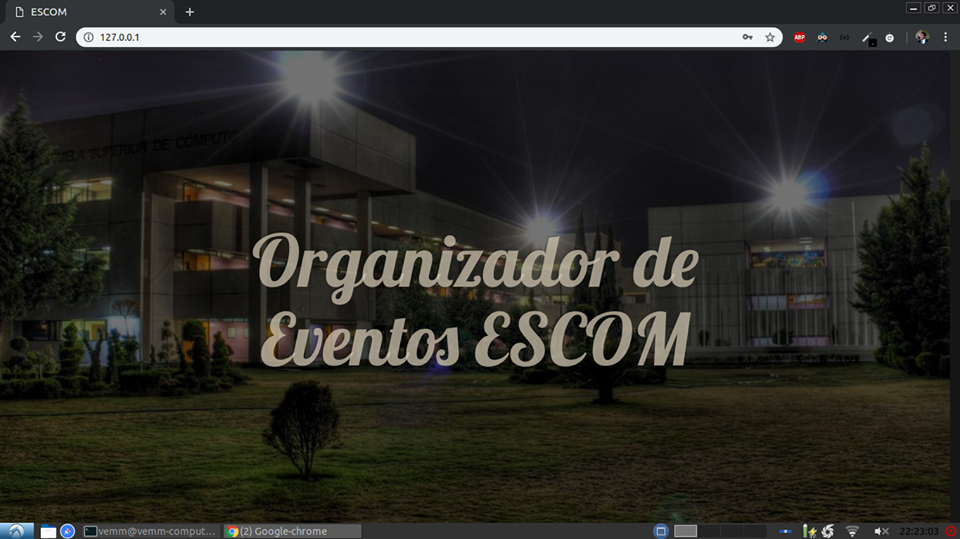
\includegraphics[width=9cm]{./img/lista/1.png}
				\caption[Acceso a contenedor virtual por IP]{Acceso a contenedor virtual por IP}
				\label{fig:1}
			\end{figure}
			\begin{figure}[htbp]
			\centering
				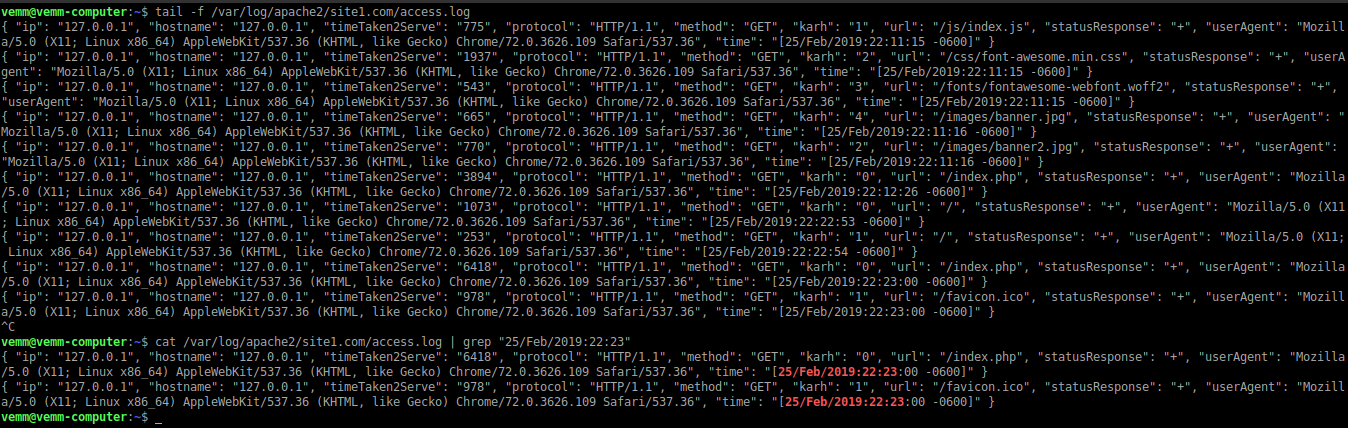
\includegraphics[width=9cm]{./img/lista/1_1.png}
				\label{fig:1.1}
			\end{figure}
		\item Acceso a contenedor virtual por dominio.
			\begin{figure}[htbp]
				\centering
				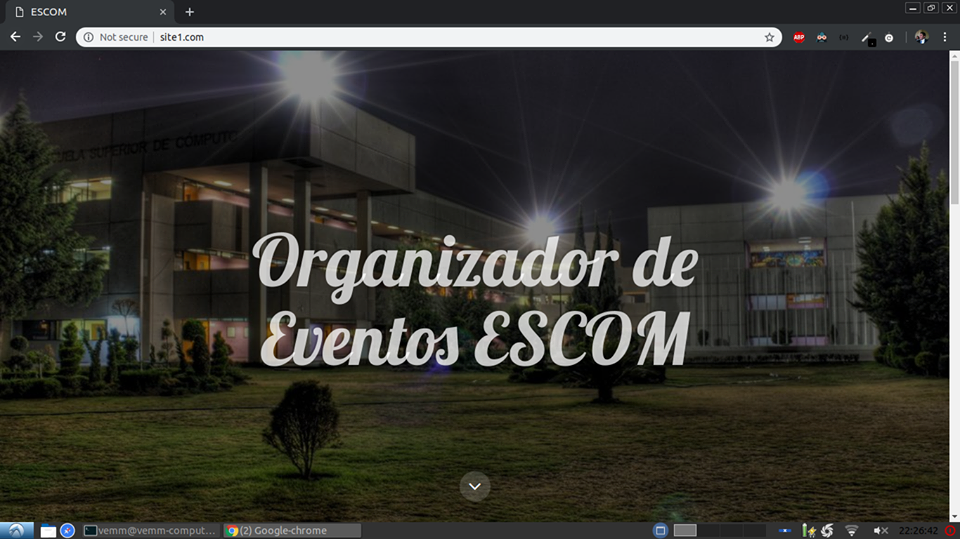
\includegraphics[width=9cm]{./img/lista/2.png}
				\caption[Acceso a contenedor virtual por dominio]{Acceso a contenedor virtual por dominio}
				\label{fig:2}
			\end{figure}
			\begin{figure}[htbp]
			\centering
				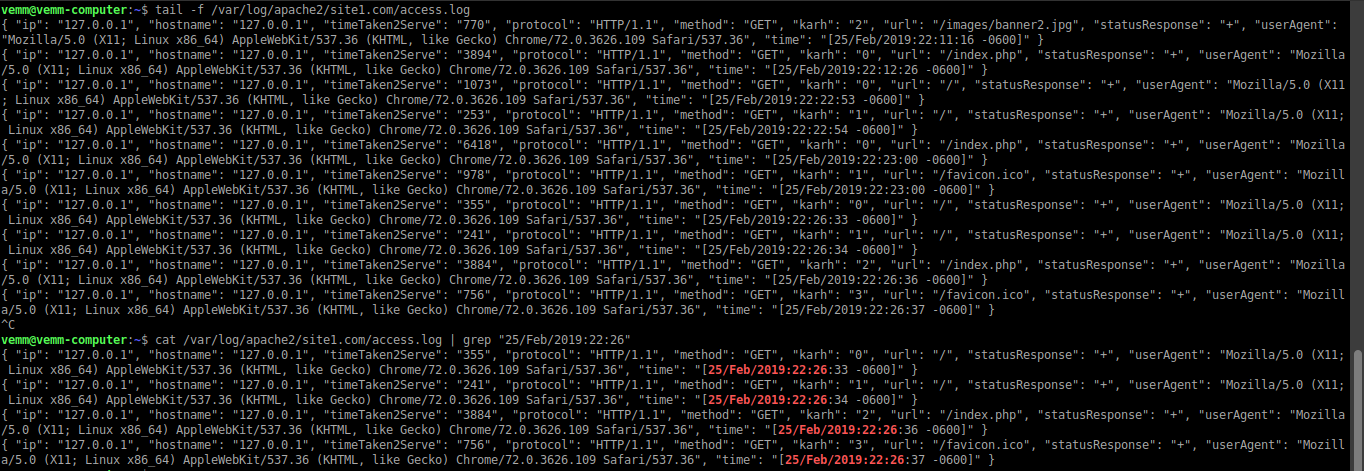
\includegraphics[width=9cm]{./img/lista/2_1.png}
				\label{fig:2.1}
			\end{figure}
	\end{enumerate}

\subsection{Restricciones de acceso}
	\begin{enumerate}
		\item Restringir acceso al recurso por dirección IP del cliente.
			\begin{figure}[htbp]
				\centering
				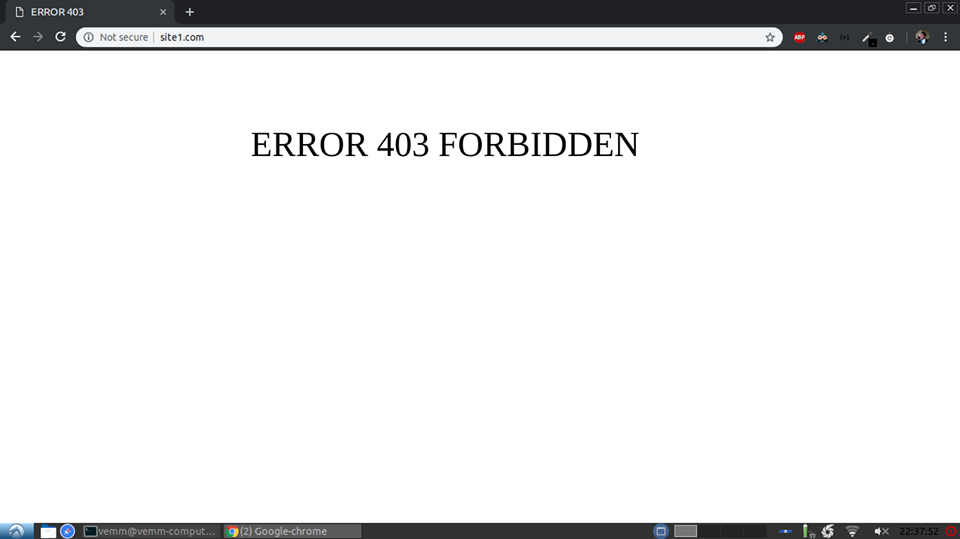
\includegraphics[width=9cm]{./img/lista/3.png}
				\caption[Restringir acceso al recurso por dirección IP del cliente]{Restringir acceso al recurso por dirección IP del cliente}
				\label{fig:3}
			\end{figure}
			\begin{figure}[htbp]
			\centering
				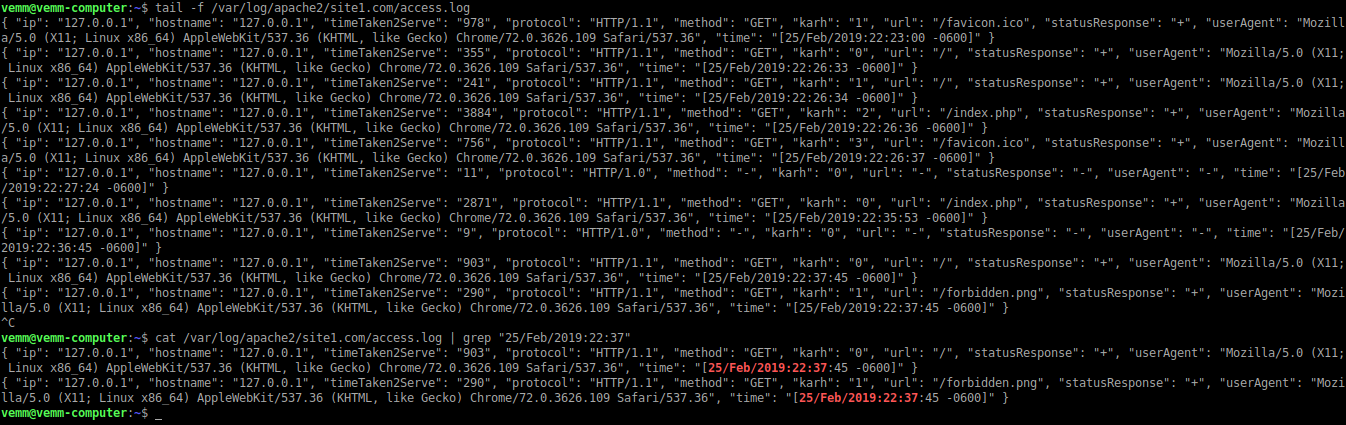
\includegraphics[width=9cm]{./img/lista/3_1.png}
				\label{fig:3.1}
			\end{figure}
		\item Restringir acceso al recurso por segmento de red\\
			\begin{figure}[htbp]
				\centering
				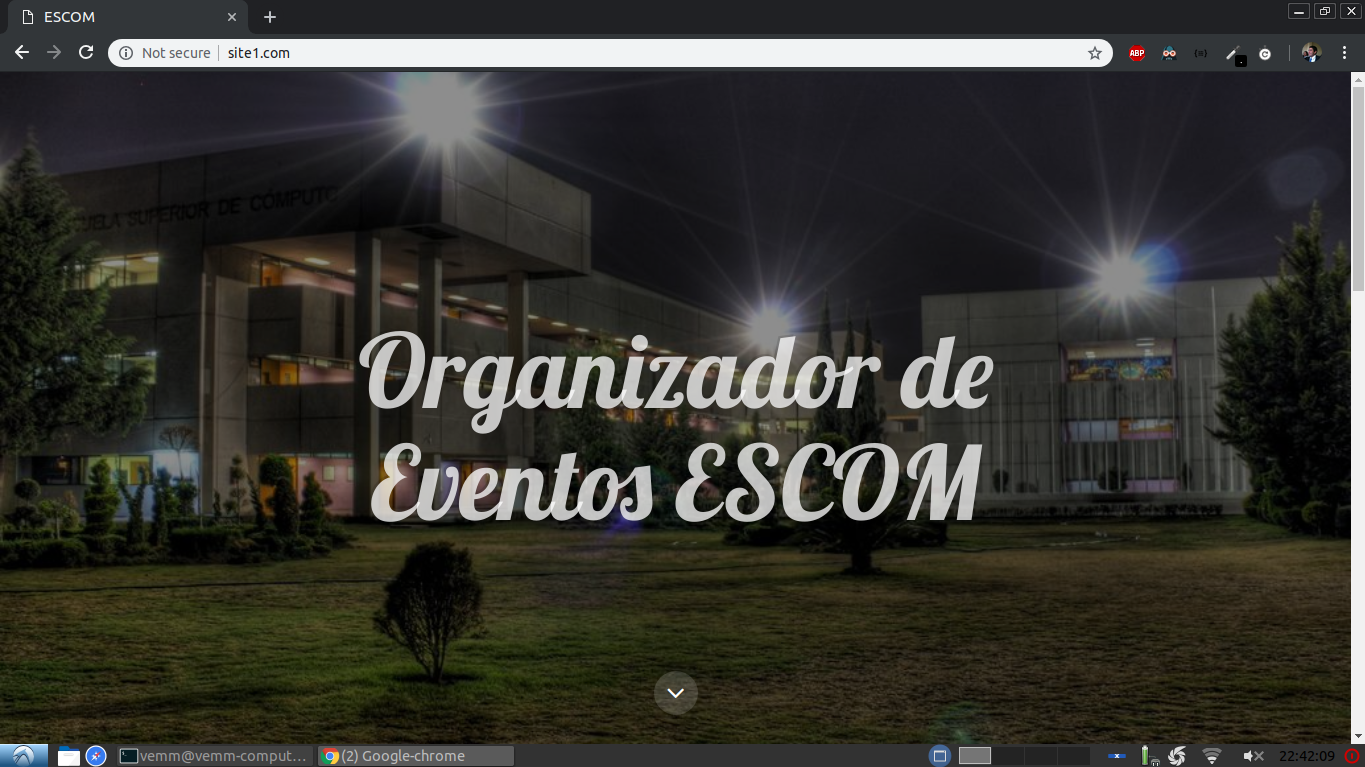
\includegraphics[width=9cm]{./img/lista/4.png}
				\caption[Restringir acceso al recurso por segmento de red]{Restringir acceso al recurso por segmento de red}
				\label{fig:4}
			\end{figure}
			\begin{figure}[htbp]
			\centering
				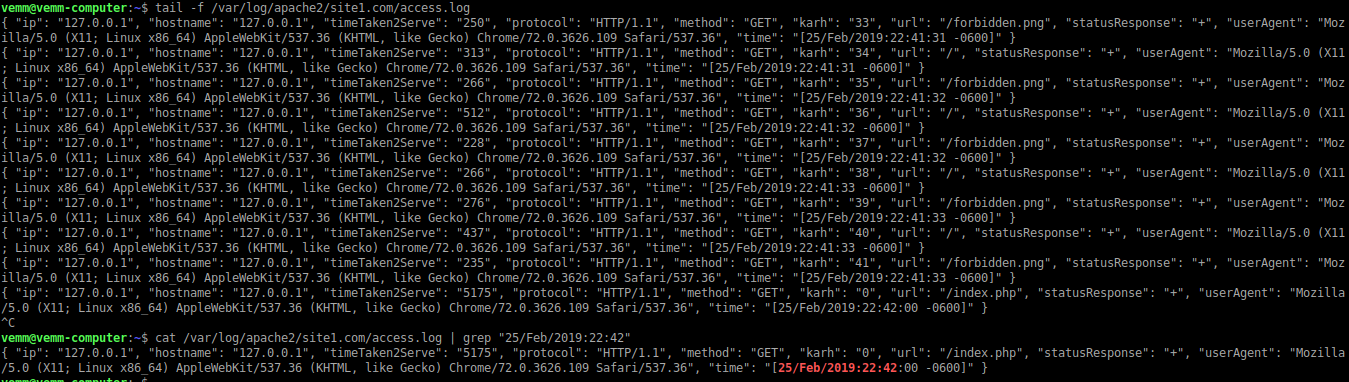
\includegraphics[width=9cm]{./img/lista/4_1.png}
				\label{fig:4.1}
			\end{figure}
		\item Restringir acceso al recurso por nombre de usuario (grupo de usuarios)/clave de acceso.
			\begin{figure}[htbp]
				\centering
				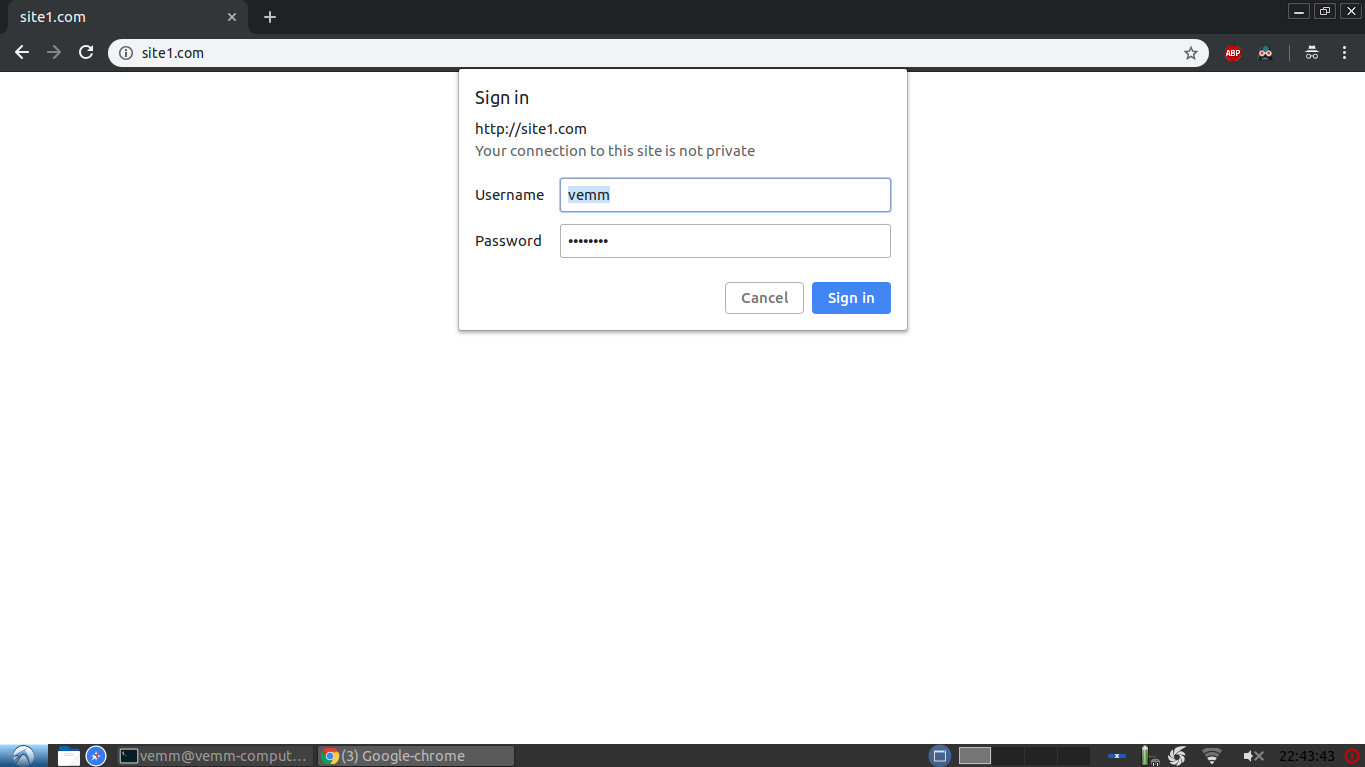
\includegraphics[width=9cm]{./img/lista/5.png}
				\caption[Restringir acceso al recurso por nombre de usuario (grupo de usuarios)/clave de acceso]{Restringir acceso al recurso por nombre de usuario (grupo de usuarios)/clave de acceso}
				\label{fig:5}
			\end{figure}
			\begin{figure}[htbp]
			\centering
				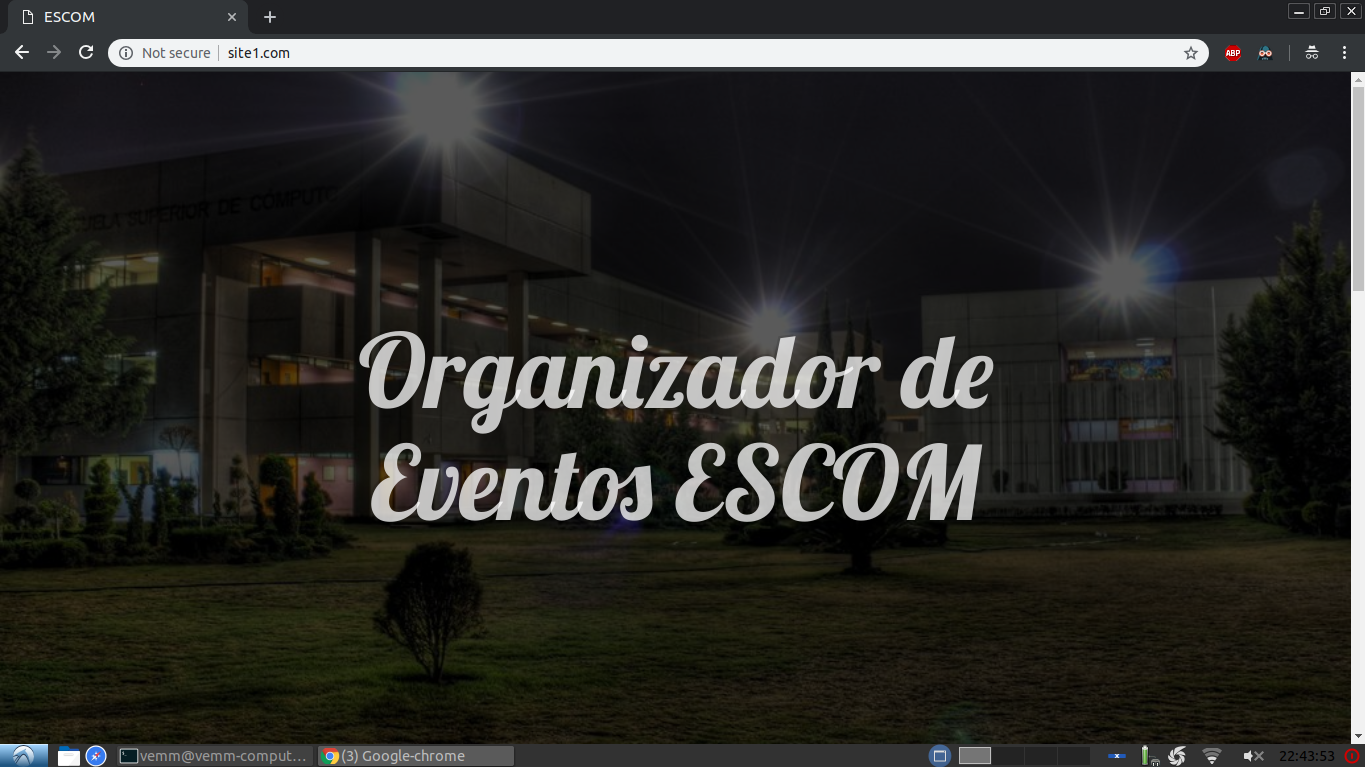
\includegraphics[width=9cm]{./img/lista/5_1.png}
				\label{fig:5.1}
			\end{figure}
			\begin{figure}[htbp]
			\centering
				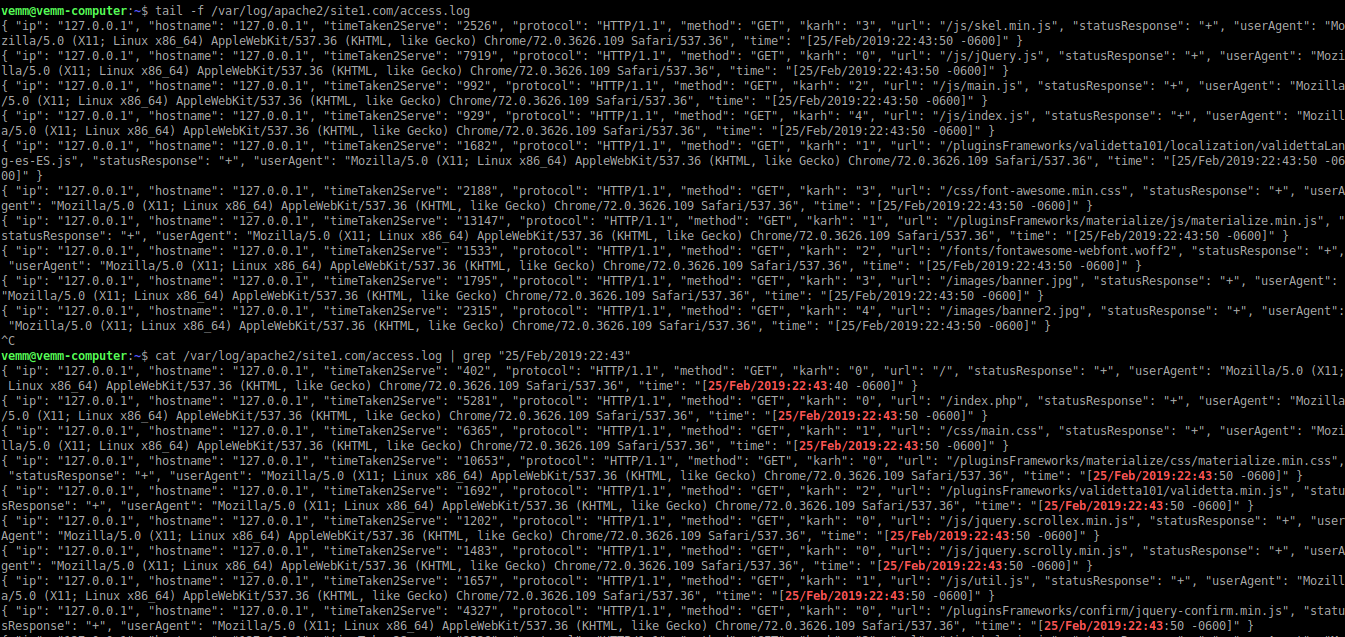
\includegraphics[width=9cm]{./img/lista/5_2.png}
				\label{fig:5.2}
			\end{figure}
	\end{enumerate}

\subsection{Configuración de servicio con seguridad en el transporte}
	\begin{enumerate}
		\item Configuración de puerto de operación.
			\begin{figure}[htbp]
				\centering
				
\includegraphics[width=9cm]{./img/lista/6.png}
				\caption[Configuración de puerto de operación]{Configuración de puerto de operación}
				\label{fig:6}
			\end{figure}
			\begin{figure}[htbp]
			\centering
				
\includegraphics[width=9cm]{./img/lista/6_1.png}
				\label{fig:6.1}
			\end{figure}
			\begin{figure}[htbp]
			\centering
				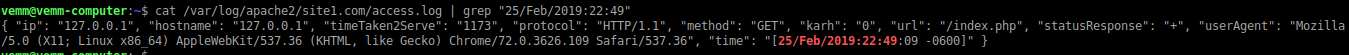
\includegraphics[width=9cm]{./img/lista/6_2.png}
				\label{fig:6.2}
			\end{figure}
		\item Servidor de aplicación utilizando el protocolo HTTPS.
			\begin{figure}[htbp]
				\centering
				
\includegraphics[width=9cm]{./img/lista/7.png}
				\caption[Servidor de aplicación utilizando el protocolo HTTPS]{Servidor de aplicación utilizando el protocolo HTTPS}
				\label{fig:7}
			\end{figure}
			\begin{figure}[htbp]
			\centering
				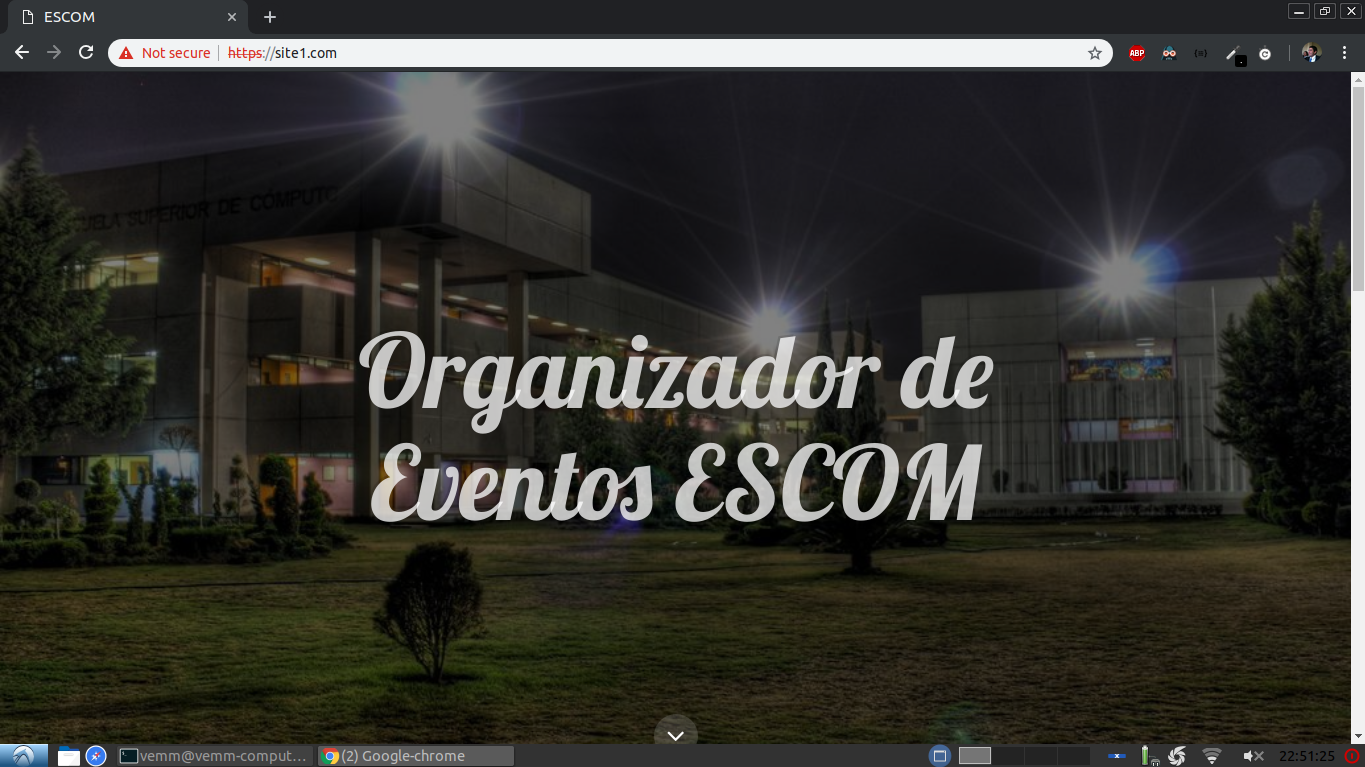
\includegraphics[width=9cm]{./img/lista/7_1.png}
				\label{fig:7.1}
			\end{figure}
			\begin{figure}[htbp]
			\centering
				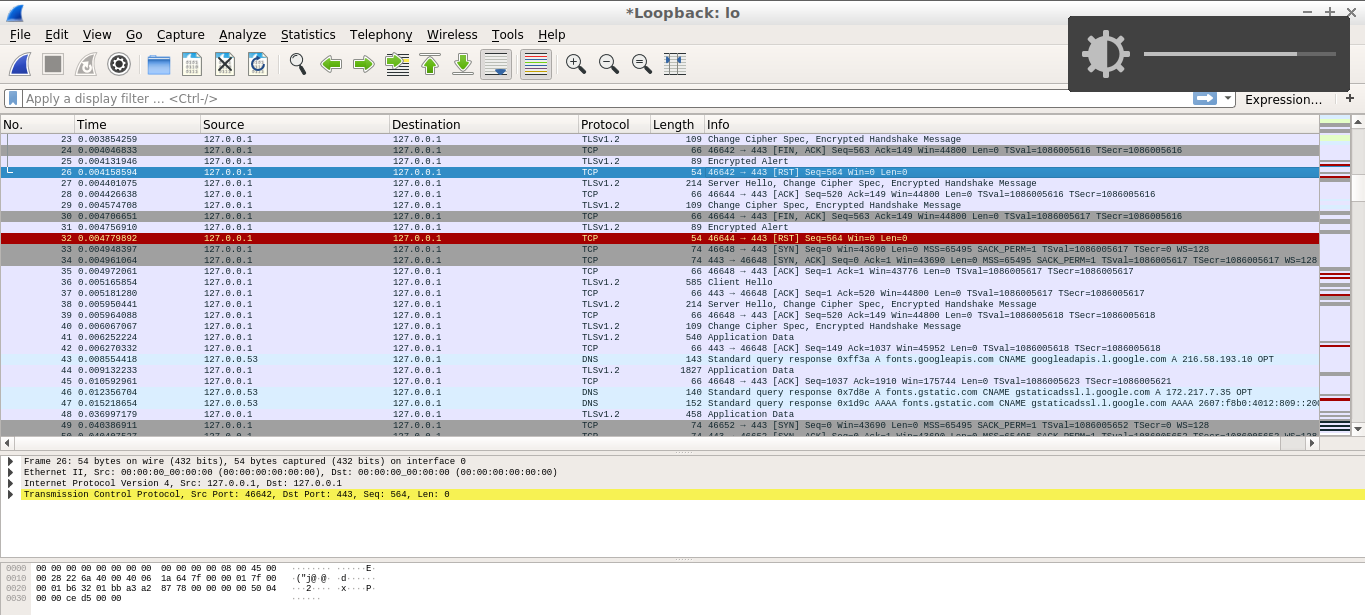
\includegraphics[width=9cm]{./img/lista/7_2.png}
				\label{fig:7.2}
			\end{figure}
			\begin{figure}[htbp]
			\centering
				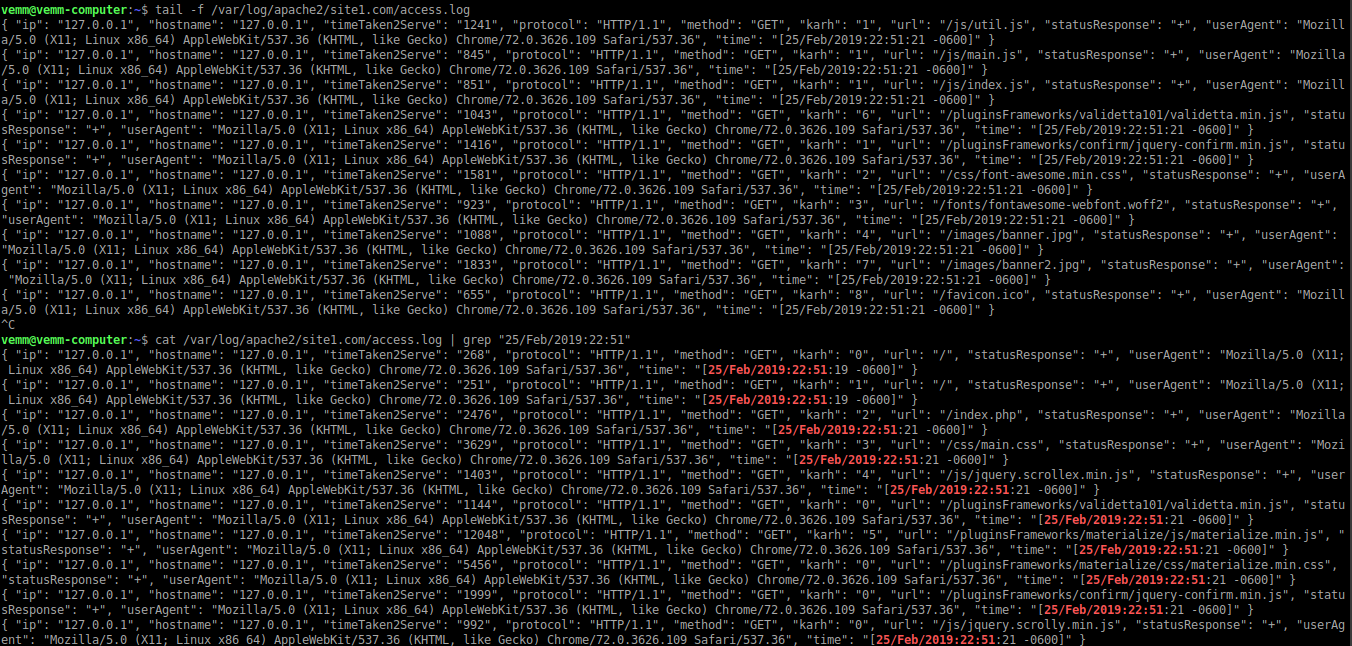
\includegraphics[width=9cm]{./img/lista/7_3.png}
				\label{fig:7.3}
			\end{figure}
		\item Definición de certificados /llaves de operación.
			\begin{figure}[htbp]
				\centering
			
				\caption[Definición de certificados /llaves de operación]{Definición de certificados /llaves de operación}
				\label{fig:8}
			\end{figure}
		\item Certificados auto firmados.
			\begin{figure}[htbp]
				\centering
				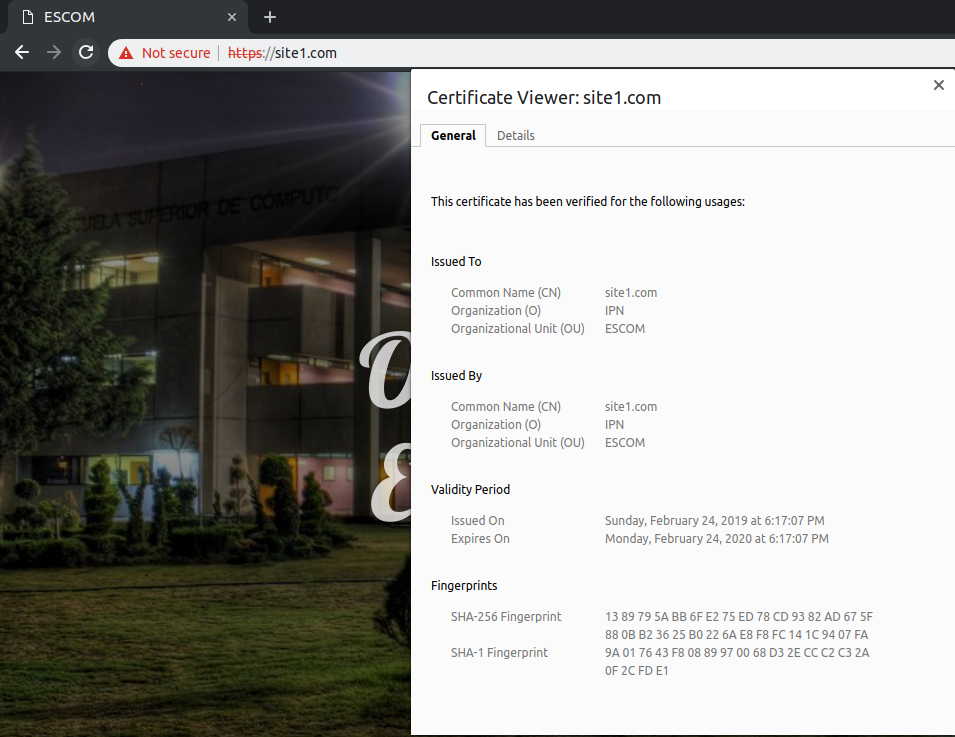
\includegraphics[width=9cm]{./img/lista/9.png}
				\caption[Certificados auto firmados]{Certificados auto firmados}
				\label{fig:9}
			\end{figure}
		\item Certificados firmados por un tercero (Autoridad certificadora)
			\begin{figure}[htbp]
				\centering
				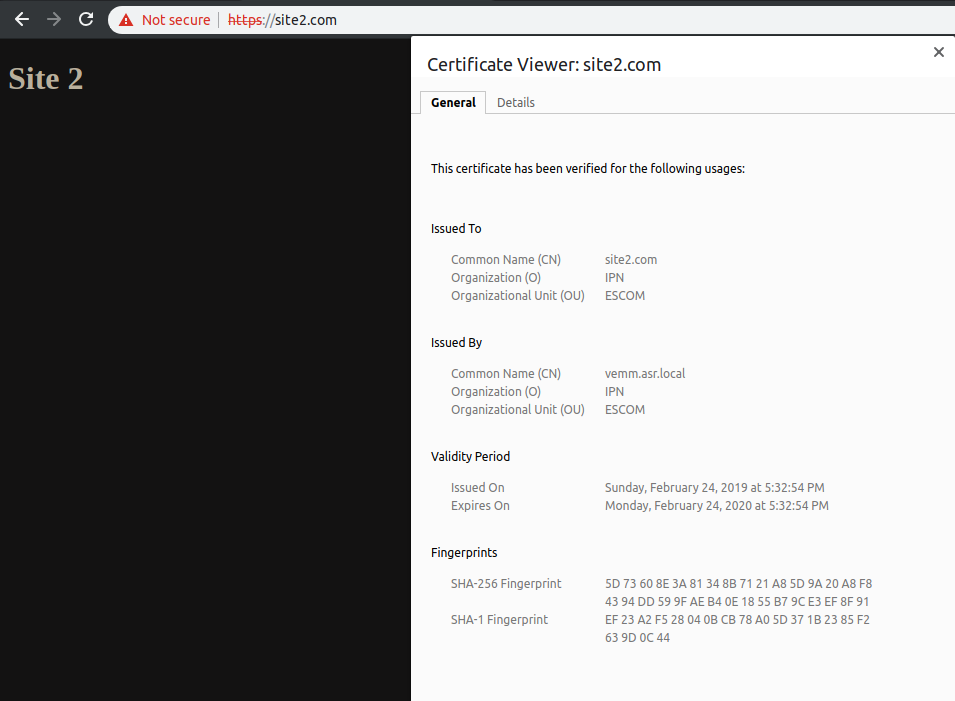
\includegraphics[width=9cm]{./img/lista/10.png}
				\caption[Certificados firmados por un tercero (Autoridad certificadora)]{Certificados firmados por un tercero (Autoridad certificadora)}
				\label{fig:10}
			\end{figure}
		\item Trama de elemento cifrado
			\begin{figure}[htbp]
				\centering
				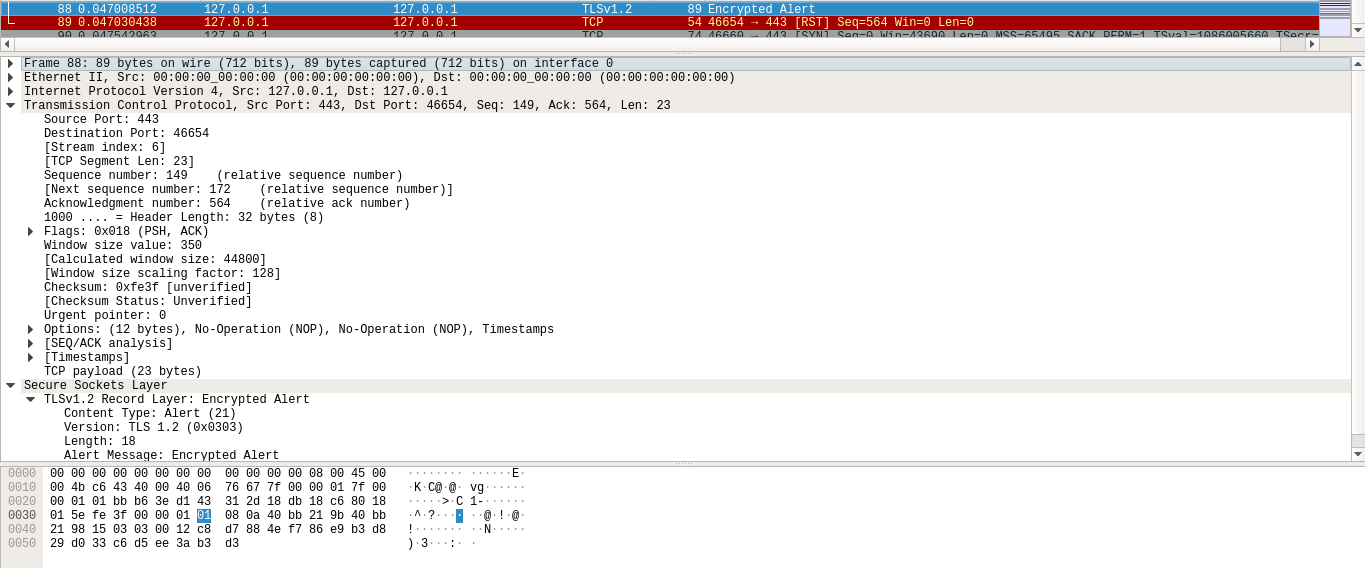
\includegraphics[width=9cm]{./img/lista/11.png}
				\caption[Trama de elemento cifrado]{Trama de elemento cifrado}
				\label{fig:11}
			\end{figure}
	\end{enumerate}

\subsection{Personalización de páginas de error}
	\begin{enumerate}
		\item Error 1: Tipo y muestra.
			\begin{figure}[htbp]
				\centering
				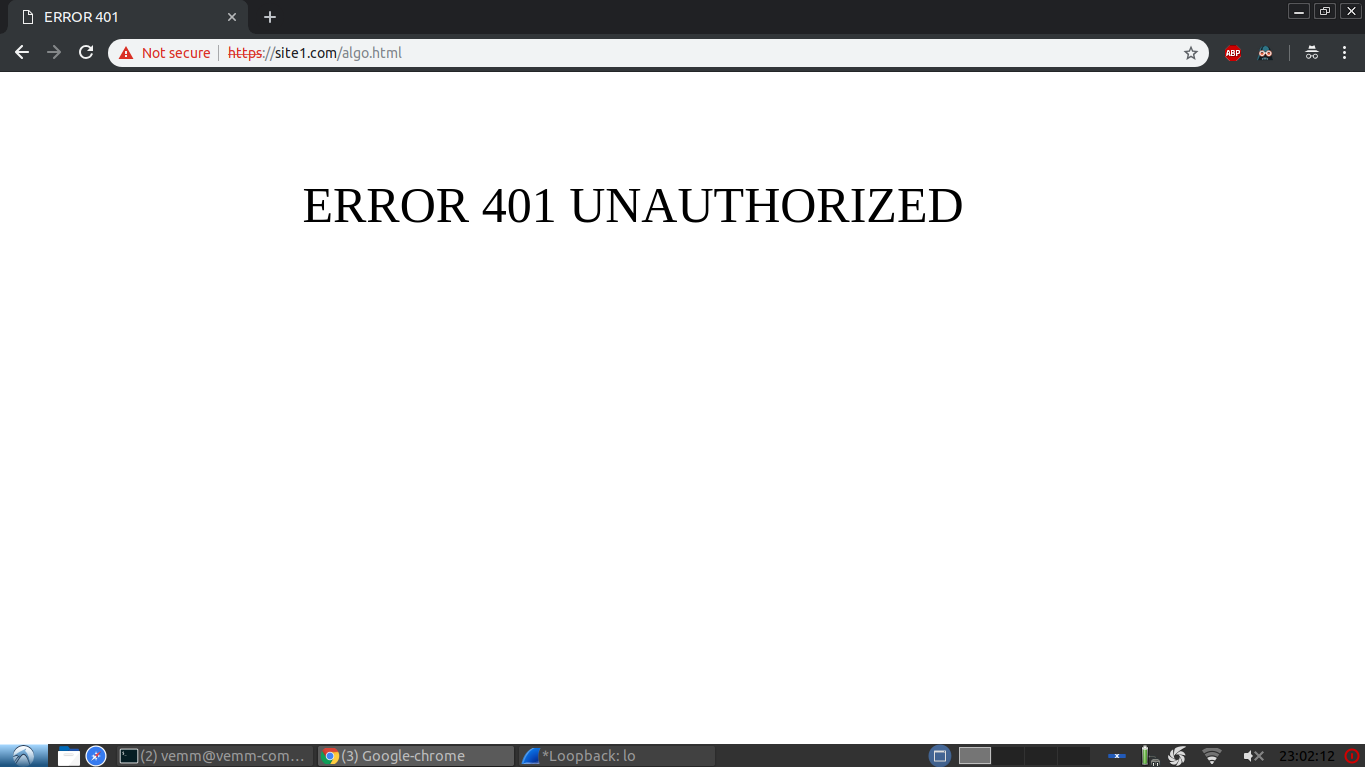
\includegraphics[width=9cm]{./img/lista/12.png}
				\caption[Error 1: Tipo y muestra]{Error 1: Tipo y muestra}
				\label{fig:12}
			\end{figure}
			\begin{figure}[htbp]
			\centering
				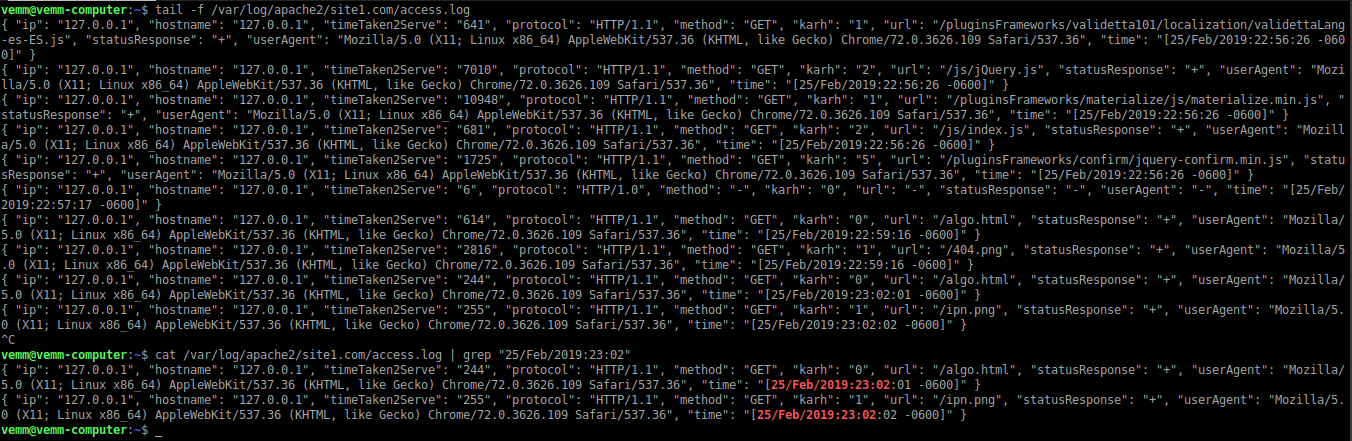
\includegraphics[width=9cm]{./img/lista/12_1.png}
				\label{fig:12.1}
			\end{figure}
		\item Error 2: Tipo y muestra.
			\begin{figure}[htbp]
				\centering
				
\includegraphics[width=9cm]{./img/lista/13.png}
				\caption[Error 2: Tipo y muestra]{Error 2: Tipo y muestra}
				\label{fig:13}
			\end{figure}
			\begin{figure}[htbp]
			\centering
				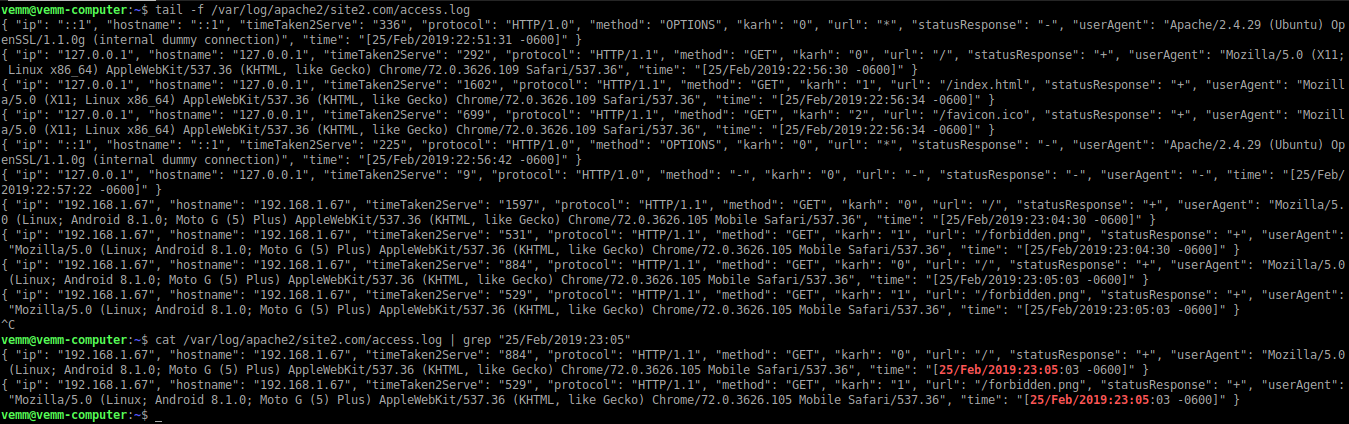
\includegraphics[width=9cm]{./img/lista/13_1.png}
				\label{fig:13.1}
			\end{figure}
		\item Error 3: Tipo y muestra.
			\begin{figure}[htbp]
				\centering
				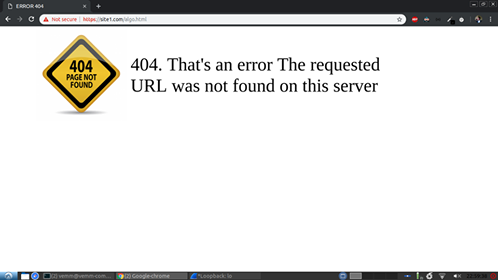
\includegraphics[width=9cm]{./img/lista/14.png}
				\caption[Error 3: Tipo y muestra]{Error 3: Tipo y muestra}
				\label{fig:14}
			\end{figure}
			\begin{figure}[htbp]
			\centering
				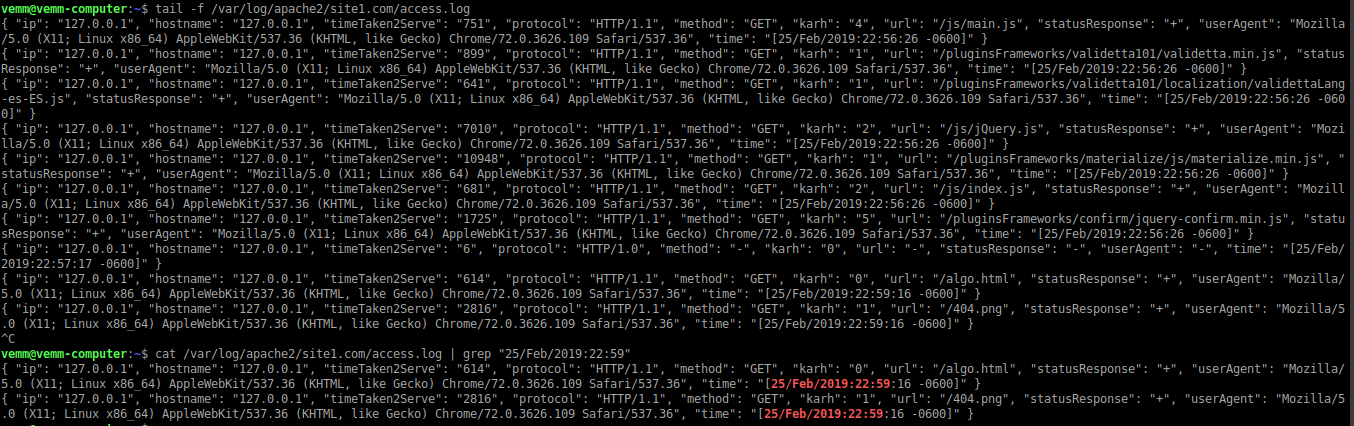
\includegraphics[width=9cm]{./img/lista/14_1.png}
				\label{fig:14.1}
			\end{figure}
	\end{enumerate}

\subsection{Configuración de archivos de bitácoras}
	\begin{enumerate}
		\item Nivel de configuración de operación y definición del tipo de dato.
			\begin{figure}[htbp]
				\centering
				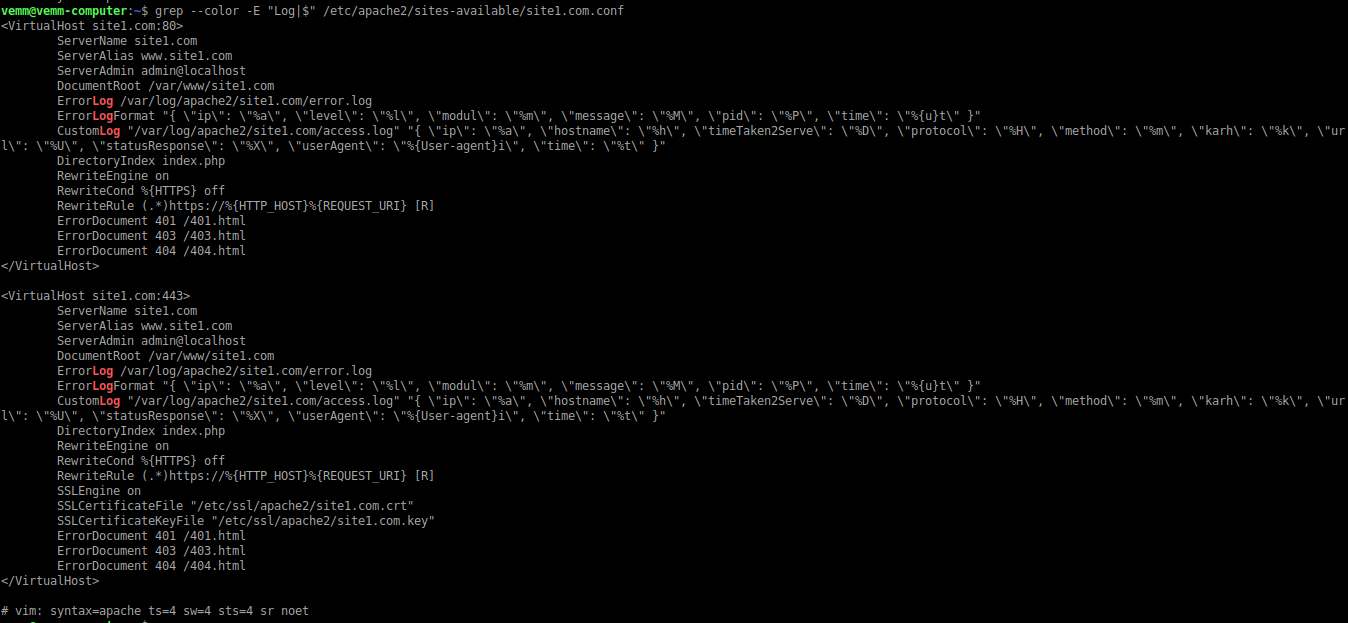
\includegraphics[width=9cm]{./img/lista/15.png}
				\caption[Certificados auto firmados]{Certificados auto firmados}
				\label{fig:15}
			\end{figure}
		\item Nivel de configuración y mensajes de error
			\begin{figure}[htbp]
				\centering
				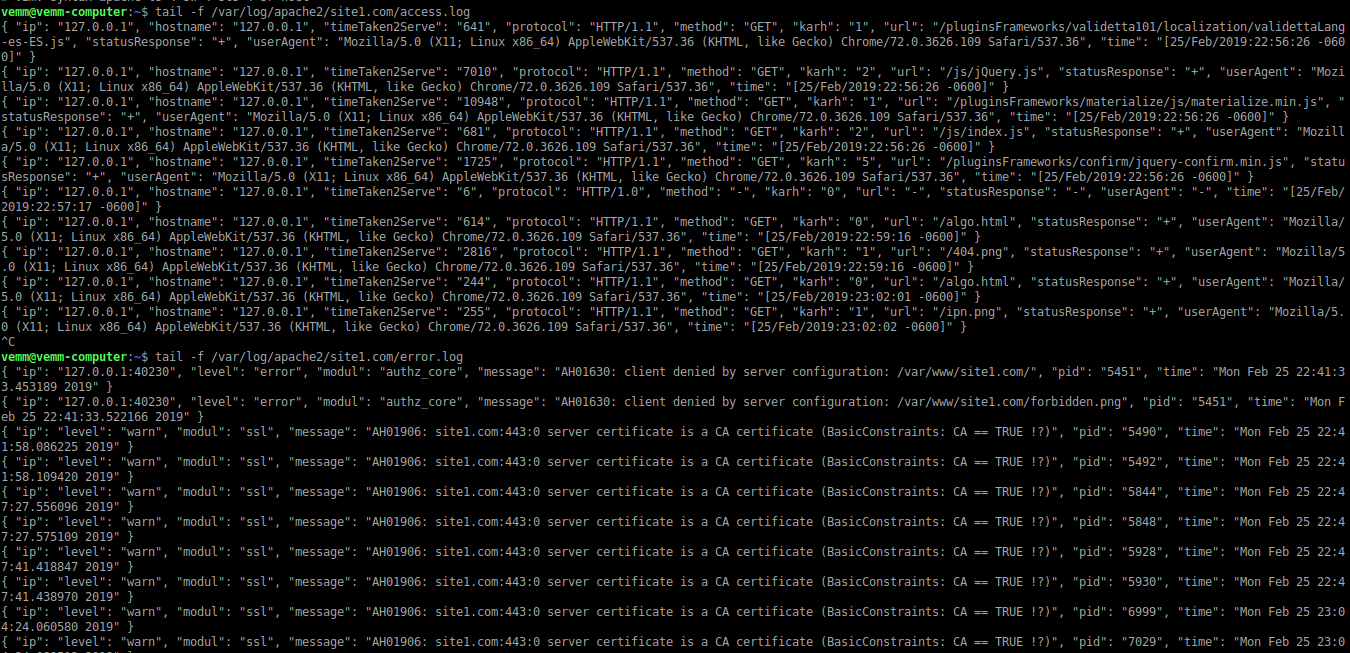
\includegraphics[width=9cm]{./img/lista/16.png}
				\caption[Nivel de configuración y mensajes de error]{Nivel de configuración y mensajes de error}
				\label{fig:16}
			\end{figure}
	\end{enumerate}

\subsection{Resumen de operación de forma dinámica (Sitios, solicitudes, estado del sistema y recursos consumidos)}
	\begin{enumerate}
		\item Configuración y módulos activados
			\begin{figure}[htbp]
				\centering
				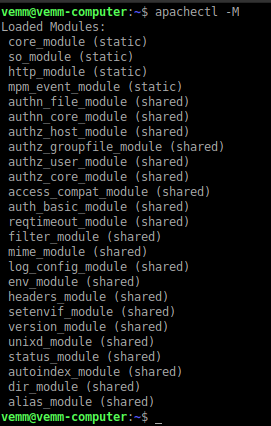
\includegraphics[width=9cm]{./img/lista/17.png}
				\caption[Configuración y módulos activados]{Configuración y módulos activados}
				\label{fig:17}
			\end{figure}
		\item Muestra de resumen de operación del servidor
		\begin{figure}[htbp]
			\centering
			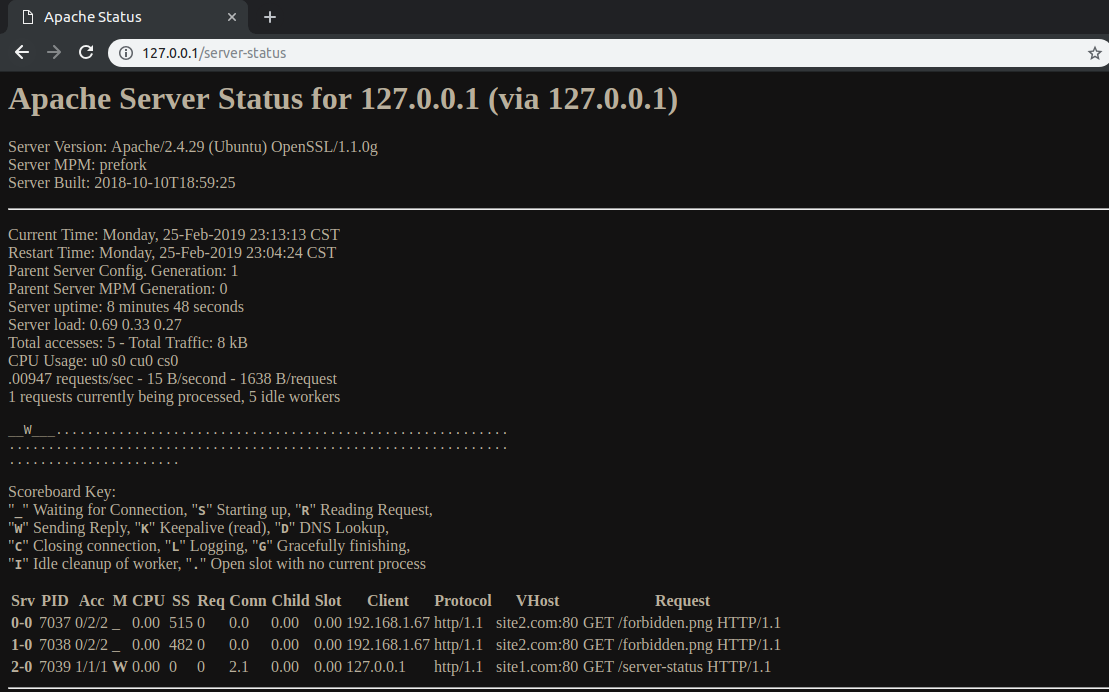
\includegraphics[width=9cm]{./img/lista/18.png}
			\caption[Muestra de resumen de operación del servidor]{Muestra de resumen de operación del servidor}
			\label{fig:18}
		\end{figure}
		\begin{figure}[htbp]
			\centering
				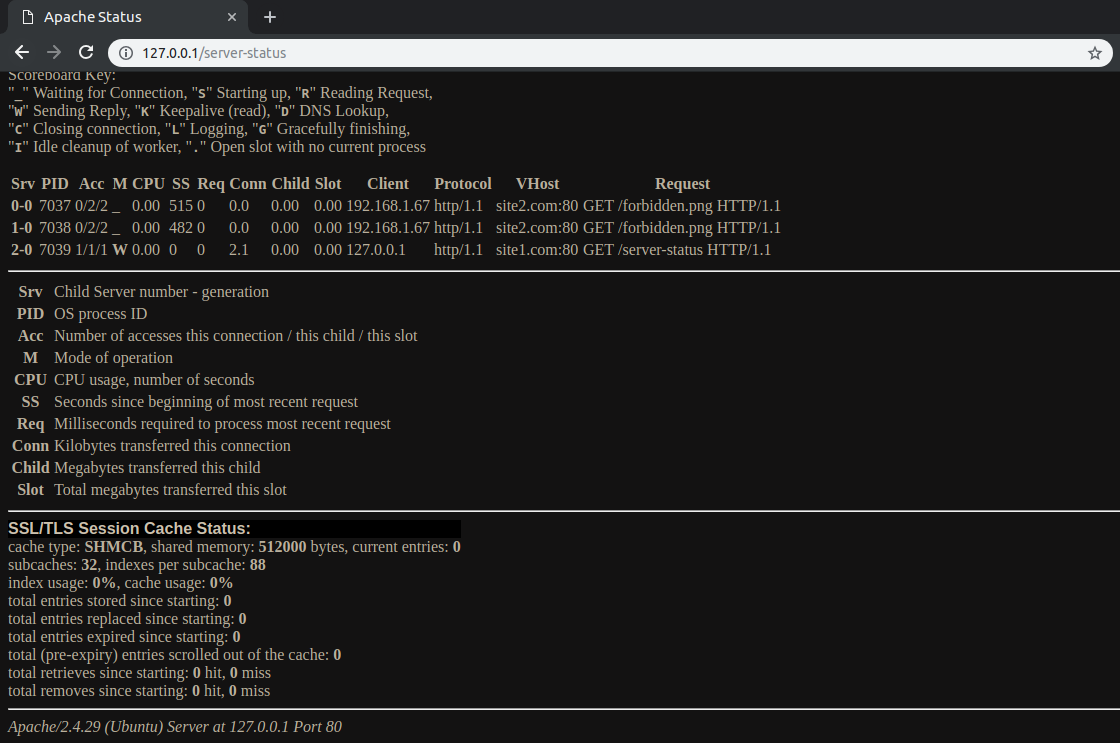
\includegraphics[width=9cm]{./img/lista/18_1.png}
				\label{fig:18.1}
			\end{figure}
	\end{enumerate}

\subsection{Tablas de resumen de operación}
	\begin{enumerate}
		\item Resumen de operación de servidor (Tabla de aplicación generada por usuario).
			\begin{figure}[htbp]
				\centering
				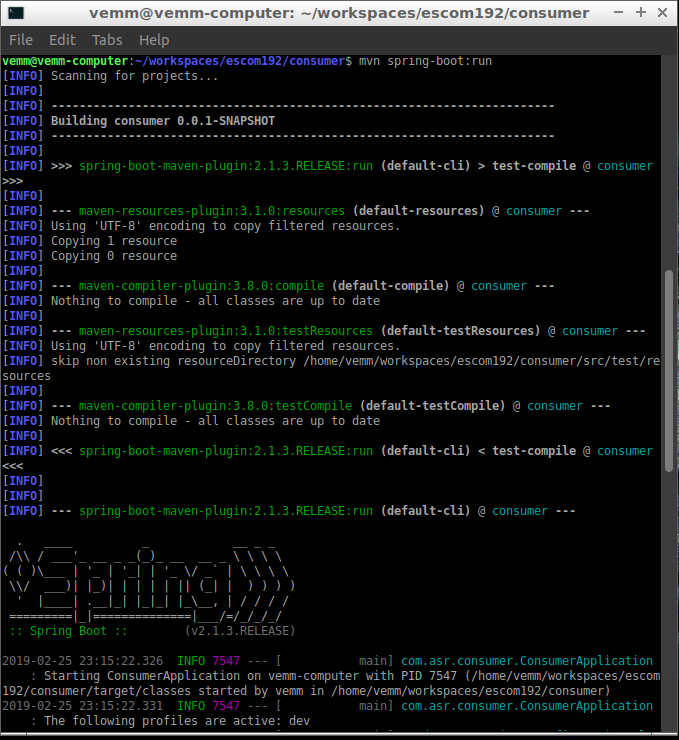
\includegraphics[width=9cm]{./img/lista/19.png}
				\caption[Resumen de operación de servidor]{Resumen de operación de servidor}
				\label{fig:19}
			\end{figure}
			\begin{figure}[htbp]
			\centering
				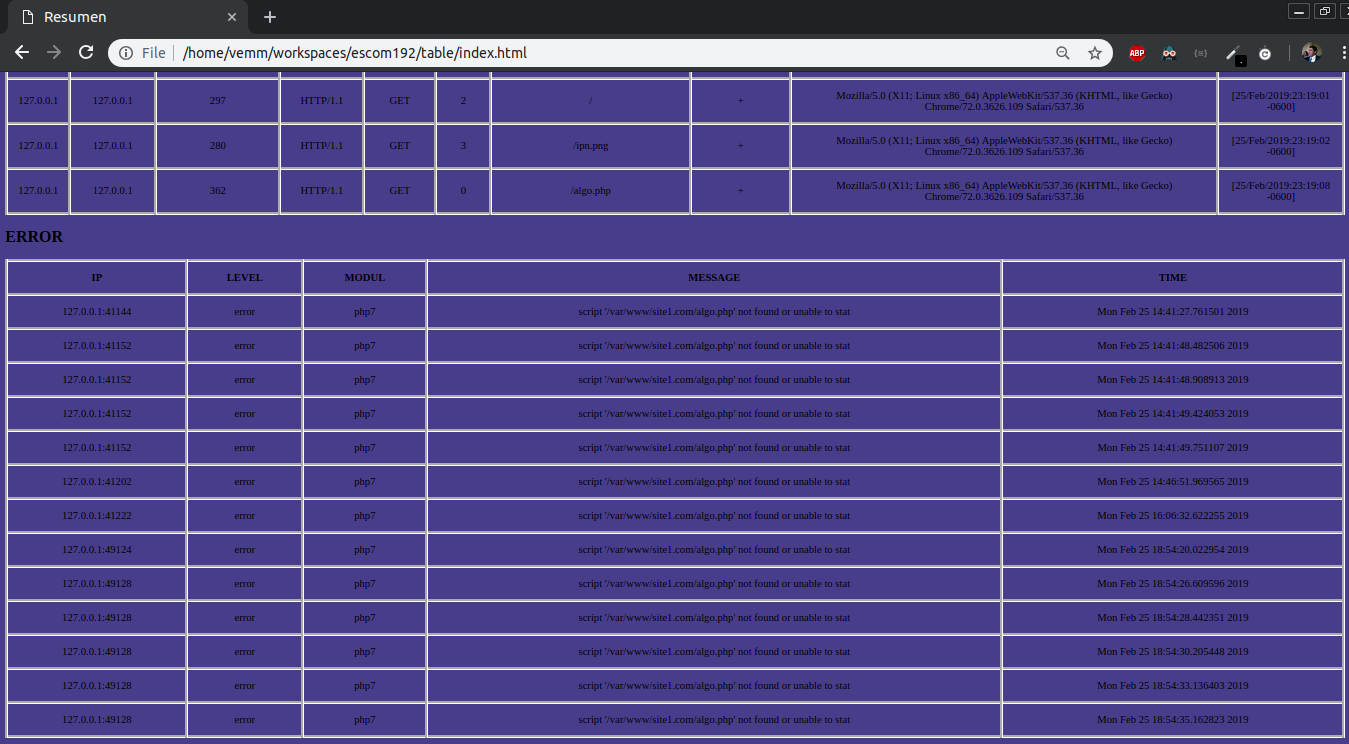
\includegraphics[width=9cm]{./img/lista/19_1.png}
				\label{fig:19.1}
			\end{figure}
		\item Resumen de errores del servidor (Tabla de aplicación generada por usuario)
			\begin{figure}[htbp]
				\centering
				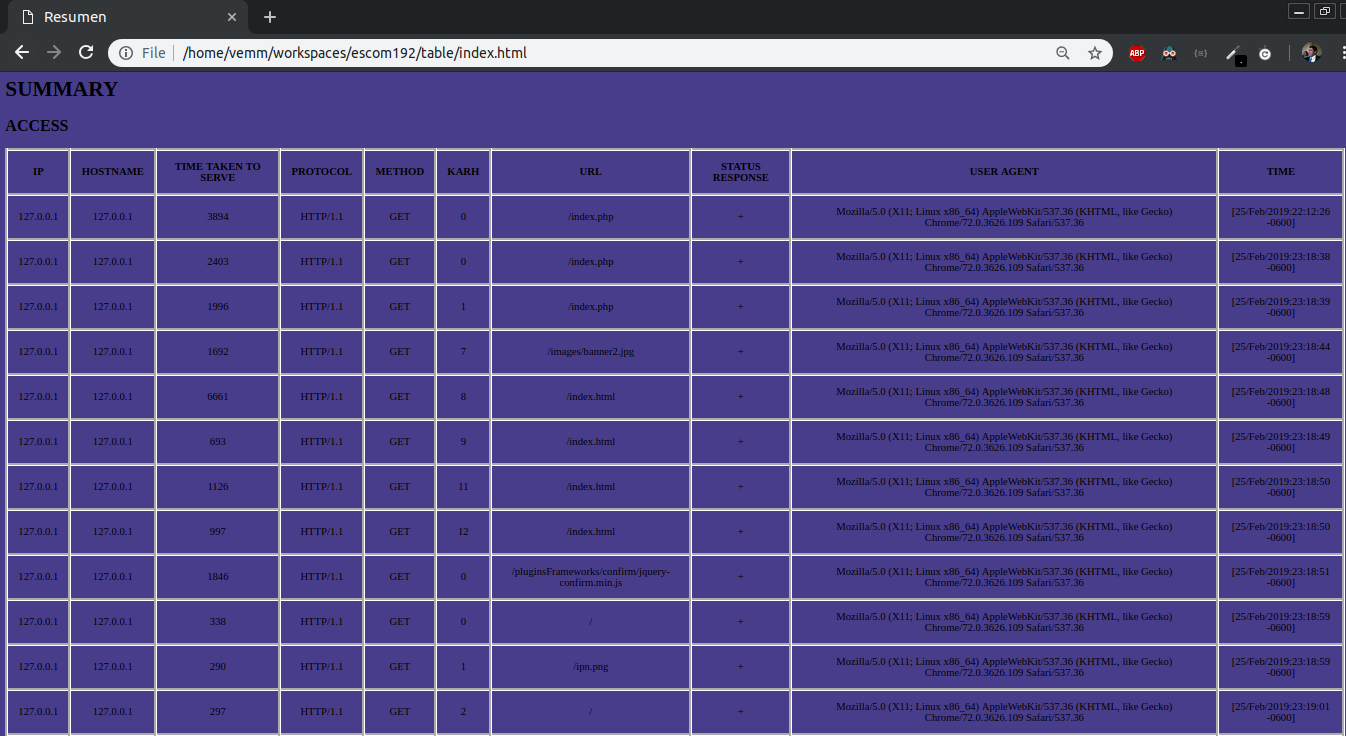
\includegraphics[width=9cm]{./img/lista/20.png}
				\caption[Resumen de errores del servidor]{Resumen de errores del servidor}
				\label{fig:20}
			\end{figure}
			\begin{figure}[htbp]
			\centering
				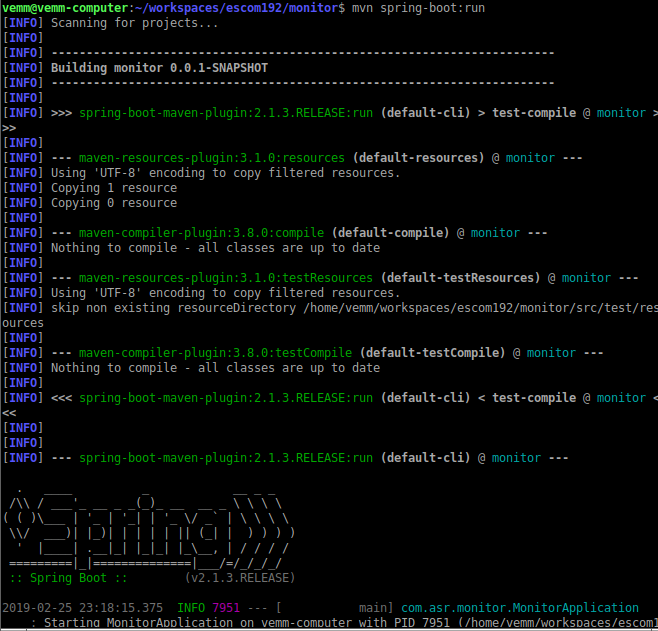
\includegraphics[width=9cm]{./img/lista/20_1.png}
				\label{fig:20.1}
			\end{figure}
	\end{enumerate}